%%%%%%%%%%%%%%%%%%%%%%%%%%%%%%%%%%%%%%%%%
% Journal Article
% LaTeX Template
% Version 1.4 (15/5/16)
%
% This template has been downloaded from:
% http://www.LaTeXTemplates.com
%
% Original author:
% Frits Wenneker (http://www.howtotex.com) with extensive modifications by
% Vel (vel@LaTeXTemplates.com)
%
% License:
% CC BY-NC-SA 3.0 (http://creativecommons.org/licenses/by-nc-sa/3.0/)
%
%%%%%%%%%%%%%%%%%%%%%%%%%%%%%%%%%%%%%%%%%

%----------------------------------------------------------------------------------------
%	PACKAGES AND OTHER DOCUMENT CONFIGURATIONS
%----------------------------------------------------------------------------------------

%\documentclass[twoside,twocolumn]{article}
\documentclass[twoside,onecolumn]{article}

\usepackage{blindtext} % Package to generate dummy text throughout this template 
\usepackage{graphicx}
\usepackage{float}
\usepackage[sc]{mathpazo} % Use the Palatino font
\usepackage[T1]{fontenc} % Use 8-bit encoding that has 256 glyphs
\linespread{1.05} % Line spacing - Palatino needs more space between lines
\usepackage{microtype} % Slightly tweak font spacing for aesthetics

\usepackage[english]{babel} % Language hyphenation and typographical rules

\usepackage[hmarginratio=1:1,top=32mm,columnsep=20pt]{geometry} % Document margins
\usepackage[hang, small,labelfont=bf,up,textfont=it,up]{caption} % Custom captions under/above floats in tables or figures
\usepackage{booktabs} % Horizontal rules in tables

\usepackage{lettrine} % The lettrine is the first enlarged letter at the beginning of the text

\usepackage{enumitem} % Customized lists
\setlist[itemize]{noitemsep} % Make itemize lists more compact

\usepackage{abstract} % Allows abstract customization
\renewcommand{\abstractnamefont}{\normalfont\bfseries} % Set the "Abstract" text to bold
\renewcommand{\abstracttextfont}{\normalfont\small\itshape} % Set the abstract itself to small italic text

%\usepackage{titlesec} % Allows customization of titles
%\renewcommand\thesection{\Roman{section}} % Roman numerals for the sections
%\renewcommand\thesubsection{\roman{subsection}} % roman numerals for subsections
%\titleformat{\section}[block]{\large\scshape\centering}{\thesection.}{1em}{} % Change the look of the section titles
%\titleformat{\subsection}[block]{\large}{\thesubsection.}{1em}{} % Change the look of the section titles

\usepackage{fancyhdr} % Headers and footers
\pagestyle{fancy} % All pages have headers and footers
\fancyhead{} % Blank out the default header
\fancyfoot{} % Blank out the default footer
\cfoot{\thepage}

%\fancyhead[C]{Running title $\bullet$ May 2016 $\bullet$ Vol. XXI, No. 1} % Custom header text
%\fancyfoot[RO,LE]{\thepage} % Custom footer text

\usepackage{titling} % Customizing the title section

\usepackage{hyperref} % For hyperlinks in the PDF
\usepackage{cases}

%----------------------------------------------------------------------------------------
%	TITLE SECTION
%----------------------------------------------------------------------------------------

\setlength{\droptitle}{-4\baselineskip} % Move the title up

\pretitle{\begin{center}\Huge\bfseries} % Article title formatting
\posttitle{\end{center}} % Article title closing formatting
%\title{Modelling Zero-inflated Count Data with Expectation-Maximization Algorithm with Application to Regulatory Compliance} % Article title
\title{A Bayesian Approach for Modelling Zero-Inflated Count Data with an Application in Regulatory Compliance} % Article title
\author{%
\textsc{Michael Hur} \\[1ex] % Your name
%\normalsize Department of Statistics and Actuarial Science \\ % Your institution
%\normalsize University of Waterloo \\ % Your institution
\normalsize \href{mailto:jhhur@uwaterloo.ca}{jhhur (at) uwaterloo.ca} % Your email address
%\and % Uncomment if 2 authors are required, duplicate these 4 lines if more
%\textsc{Jane Smith}\thanks{Corresponding author} \\[1ex] % Second author's name
%\normalsize University of Utah \\ % Second author's institution
%\normalsize \href{mailto:jane@smith.com}{jane@smith.com} % Second author's email address
}
\date{} % Leave empty to omit a date
\renewcommand{\maketitlehookd}{%
\begin{abstract}
When analysing the count data, it is common to encounter the zero-inflated data where the standard regression approach is not applicable. Regulatory compliance is one area in which the compliance data that the regulatory agencies collect from inspecting the regulated businesses is often zero-inflated. To address the problem of over-dispersion, many approaches including zero-inflated Poisson regression and hurdle model have been introduced. While these approaches comprise of the mixture model, it is often difficult for the business user to understand the nature of the mixture model and correctly utilize the available methods. This paper introduces a Bayesian approach for the zero-inflated count data which incorporates prior information and allows an easy implementation in practice.
\end{abstract}
}

%----------------------------------------------------------------------------------------

\begin{document}

% Print the title
\maketitle

%----------------------------------------------------------------------------------------
%	ARTICLE CONTENTS
%----------------------------------------------------------------------------------------

\section{Introduction}
Compliance and inspections are major functions of regulatory agencies and any greater details into how infractions arise are valuable to the organizations. The value proposition is exploring data which has the potential to enhance and streamline operational activities, validate and strengthen policies, and provide foundational evidence to further refine regulatory efforts.

Statistically modelling compliance data usually involves the analysis of count data whose distribution exhibits an excess count of zeros. The Poisson regression model is introduced as a standard approach to model count data; however, the model assumes the mean-variance relationship of the Poisson distribution; hence, it is deemed inappropriate for fitting zero-inflated count data.

Several discrete mixture models were proposed to handle the count data with excess zeros and the problem of over-dispersion it accompanies. For instance, Lambert (1992)\cite{Lambert} discusses the zero-inflated Poisson (ZIP) model which utilizes an Expectation-Maximization (EM) algorithm. The hurdle model introduced by Mullahy (1986)\cite{Mullahy} uses a mixture of a point mass at zero and a truncated count model for the non-zero values. While these models are widely used to address the zero-inflated count data, the nature of the mixture model is often difficult for the business users to understand. In this paper, we propose a Markov Chain Monte Carlo (MCMC) algorithm to address the challenge of estimating the parameters of the zero-inflated data with an application in the regulatory compliance, which comprises of the number of observed infractions by the registered establishment. 

%------------------------------------------------

\section{Description of Regulatory Compliance Data}
Toronto Public Health is a department of the City of Toronto whose responsibility is to promote healthy environment in the Greater Toronto Area (GTA). As a regulator, Toronto Public Health is charged with developing, implementing and enforcing food safety practices at the local level, which are in public interest while also being sensitive to the economic viability of industry. These policies provide the regulatory requirements for responsible sale and service of retail food in the city.

To ensure establishments are complying with provincial laws and generally providing safe and responsible services to the public, the organization inspects and monitors licensees. These duties are carried out by inspectors who are assigned to a respective area in the city to review. Inspections make up a sizeable part of the regulator's front-line operational services and require a deep understanding not only of food safety requirements but also how establishments behave in practice. The role combines complex government knowledge with street smarts in the pursuit of mitigating risk to patrons and the general public. While the current inspectors are very capable and do an exceptional job enforcing the regulations, infractions and non-compliance still persists. While infractions will never be wholly eliminated and inspectors currently have a vast array of tools to work with, any added predictive modelling enhancements could be useful in further reducing non-compliance.

The data used for this project was acquired from the City of Toronto's Open Data Catalogue\footnote{\url{https://www1.toronto.ca/wps/portal/contentonly?vgnextoid=1a66e03bb8d1e310VgnVCM10000071d60f89RCRD}}. The data is presented at the infraction level. That is, each instance of infraction is recorded along with the corresponding inspection and establishment information, including the unique identifier of the corresponding inspection, the unique identifier of the inspected establishment. If there were more than one infractions observed in a single inspection, each infraction was recorded as a separate entry. The data was then aggregated at the inspection- and establishment-level. The inspection-level data consists of the fields "Inspection ID", "Establishment ID", "IsED", "Minimum Inspection per year", and "Total." The establishment-level data consists of fields, "Establishment ID", "IsED", "Minimum Inspection per year", "Inspection", and "Total." For both dataset, the field "IsED" is an indicator for whether the establishment is in the ''Entertainment District," "Minimum Inspection per year" is the minimum number of inspections the establishment will receive in accordance with their previous compliance records, "Inspection" is the actual number of inspections conducted on the particular establishment, and "Total" is the total number of infractions observed.

This paper's primary interest lies in understanding how likely an inspection will result in a non-compliance and, if so, how many infractions will be observed. The analysis also tests the statistical significance of the "Downtown effect", a common myth that those establishment in the most populated region of the city will be more prone to unsafe practices.

%------------------------------------------------


%------------------------------------------------

\section{Model Formulation}
As demonstrated earlier, infractions are rare events such that it is needed to model the number of infractions in any given inspection using the zero-inflated model. 

\subsection{Prior Distribution}
Consider a latent Bernoulli random variable $X_{ij}$, which represents whether an establishment i in the inspection j has committed an infraction. If we denote the probability of an infraction in an inspection j by $\theta_{ij}$, we can write the probability of observing an infraction in an inspection j as follows:

\[
f(X_{ij} = x_{ij} | \theta_{ij}) = \theta_{ij}^{x_{ij}}(1-\theta_{ij})^{1-x_{ij}}
\]

where

$$
x_{ij} = 
\left\{  \begin{array}{lcl}
           1  & & \text{Infraction }\\
           0 & & \text{otherwise.}
          \end{array}
\right.
$$

\subsection{Posterior Distribution}
In order to model actual number of infractions observed at the establishment i during the inspection j, we introduce the Poisson random variable $Y_{ij}$ with the rate parameter $\psi_{ij}$. The parameter $\psi_{ij}$ can be think of as the rate at which the infraction occurs in a particular inspection j. Hence, we can write

$$
\begin{array}{rcl}
Y_{ij} | X_{ij} = 0 \sim Bernoulli(0) \\
Y_{ij} | X_{ij} = 1 \sim Poisson(\psi_{ij})
\end{array}
$$

It is easy to check that

$$
\begin{array}{rcl}
P(Y_{ij} = 0 | X_{ij} = 0)&=& 1 \\
P(Y_{ij} \geq 1 | X_{ij} = 0) &=&  0
\end{array}
$$

Similarly, in the case where the infraction is observed we can write the conditional probabilities as follows:

$$
\begin{array}{rcl}
P(Y_{ij} = y_{ij} | X_{ij} = 1) &=& \frac{\psi_{ij}^{y_{ij}} e^{-\psi_{ij}}}{y_{ij}!}
\end{array}
$$
where $y_{ij} \ge 1$.

Hence, the marginal distribution of $Y_{ij}$ can found using the latent variable $X_{ij}$. For instance,

$$
\begin{array}{rcl}
P(Y_{ij} = 0) &=& P(Y_{ij} = 0 | X_{ij} = 0)P(X_{ij} = 0) \\ &+& P(Y_{ij} = 0 | X_{ij} = 1)P(X_{ij} = 1) \\
&=& (1-\theta_{ij}) + \theta_{ij} e^{-\psi_{ij}}
\end{array}
$$

$$
\begin{array}{rcl}
P(Y_{ij} = 1) &=& P(Y_{ij} = 1 | X_{ij} = 1)P(X_{ij} = 1) \\
&=& \theta_{ij} \psi_{ij} e^{-\psi_{ij}}
\end{array}
$$

$$
\begin{array}{rcl}
P(Y_{ij} = 2) &=& P(Y_{ij} = 2 | X_{ij} = 1)P(X_{ij} = 1) \\
&=& \theta_{ij} \frac{\psi_{ij}^2 e^{-\psi_{ij}}}{2}
\end{array}
$$

In general, we can write the marginal distribution of $Y_{ij}$ as follows:

$$
P(Y_{ij} = y_{ij}) = 
\left\{  \begin{array}{lcl}
           (1-\theta_{ij}) + \theta_{ij} e^{-\psi_{ij}}  & & y_{ij}=0\\
           \theta_{ij} \frac{\psi_{ij}^{y_{ij}} e^{-\psi_{ij}}}{y_{ij}!} & & y_{ij} > 0
          \end{array}
\right.
$$
where $\lambda_{ij} > 0$. \\

Now consider the parameters $\theta_{ij}$ and $\psi_{ij}$. These parameters can be described through the deterministic relationships:

$$
\begin{array}{rcl}
\log(\frac{\theta_{ij}}{1-\theta_{ij}}) &=& (1 - E_{i})*\beta_i + E_{i}*\alpha_i \\
&=& \beta_i + E_{ij}*(\alpha_i - \beta_i) \\
\log(\psi_{ij}) &=& (1 - E_{i})*\delta_i + E_{i}*\lambda_i \\
&=& \delta_i + E_{ij}*(\lambda_i - \delta_i)\\
\end{array}
$$

where $E_{i}$ is an indicator variable for whether the establishment is in the ''Entertainment District.'' and $\alpha_i$, $\beta_i$, $\delta_i$ and $\lambda_i$ are the independent set of random quantities. We choose distributions for such quantities:
$$
\begin{array}{rcl}
\beta_i \sim N(\beta_0, \sigma_{\beta}^2) \\
\alpha_i \sim N(\alpha_0, \sigma_{\alpha}^2) \\
\delta_i \sim N(\delta_0, \sigma_{\delta}^2) \\
\lambda_i \sim N(\lambda_0, \sigma_{\lambda}^2)
\end{array}
$$
where  $\alpha_0$, $\beta_0$, $\delta_0$, $\lambda_0$, $\sigma_\alpha$, $\sigma_\beta$, $\sigma_{\delta}$ and $\sigma_\lambda$ are known quantities that are chosen such that we diffuse priors that reflects a lack of prior knowledge. Throughout this paper, we set the mean and standard deviation to be the mean and standard deviation of the number of observed infractions of the observed data.

Note that the offset variable in the expression $log(\psi_{ij}) = \delta_i + E_{ij}*(\lambda_i - \delta_i)$ is omitted for we are analyzing at the inspection level. This implies that the rate is per one inspection; hence, the offset variable is $log(n_{ij}) = log(1) = 0$.

\subsection{Sampling From Posterior Distribution}
We have derived the full conditional posterior distribution with all quantities involved. Gibbs sampling algorithm was employed to obtain draws from the full joint distribution.

$$
\begin{array}{rcl}
P(\alpha_i,\beta_i,\delta_i,\lambda_i) &\propto& P(y_i | \cdot) P(\alpha_i) P(\beta_i) P(\delta_i) P(\lambda_i)
\end{array}
$$

Notice that the notation $P(y_i | \cdot)$ represents the conditional density of X given all other quantities and $y_i$ represents the number of inspections performed on the establishment i.

\subsection{Full Conditional Distribution}
The full conditional probability of $\beta_i$ $\forall$ i is:

$$
\begin{array}{rcl}
P(\beta_i | \cdot) &\propto& P(y_i | \cdot) P(\beta_i) \\
&\propto& P(y_i | \cdot) exp{\frac{-(\beta_i-\beta_0)}{2\sigma_{\beta}^2}}
\end{array}
$$

An adaptive Metropolis-Hastings algorithm is used with a Gaussian proposal $N(\beta_i^{(k)}, (\tau_{\beta}^2)^{(k)}$ where $\beta_i^{(k)})$ is the simulated value from the $k^{th}$ iteration.

Similarly, the full conditional probability of $\delta_i$ $\forall$ i is:

$$
\begin{array}{rcl}
P(\delta_i | \cdot) &\propto& P(y_i | \cdot) P(\delta_i) \\
&\propto& P(y_i | \cdot) exp{\frac{-(\delta_i-\delta_0)}{2\sigma_{\delta}^2}}
\end{array}
$$

Again, an adaptive Metropolis-Hastings algorithm is used with a Gaussian proposal $N(\delta_i^{(k)}, (\tau_{\delta}^2)^{(k)})$ where $\delta_i^{(k)}$ is the simulated value from the $k^{th}$ iteration.

In the similar manner, we write the full conditional probability of $\alpha_i$ as follows:

$$
\begin{array}{rcl}
P(\alpha_i | \cdot) &\propto& P(y_i | \cdot) P(\alpha_i) \\
&\propto& P(y_i | \cdot) exp{\frac{-(\alpha_i-\alpha_0)}{2\sigma_{\alpha}^2}}
\end{array}
$$

where an adaptive Metropolis-Hastings algorithm is used with Gaussian proposals $N(\alpha_i^{(k)}, (\tau_{\alpha}^2)^{(k)})$ where $\alpha_i^{(k)}$ is the simulated value from the $k^{th}$ iteration.

Lastly, the full conditional probability of $\lambda_i$ $\forall$ i is:

$$
\begin{array}{rcl}
P(\lambda_i | \cdot) &\propto& P(y_i | \cdot) P(\lambda_i) \\
&\propto& P(y_i | \cdot) exp{\frac{-(\lambda_i-\lambda_0)}{2\sigma_{\lambda}^2}}
\end{array}
$$

Likewise, an adaptive Metropolis-Hastings algorithm is used with Gaussian proposals $N(\lambda_i^{(k)}, (\tau_{\lambda}^2)^{(k)})$ where $\lambda_i^{(k)}$ is the simulated value from the $k^{th}$ iteration. 

%------------------------------------------------

\section{Result}

\subsection{Monitoring Convergence}
Three different chains with randomly dispersed initial values were each run for 10,000 iterations with an adaptation period of 1,000 and burn-in of 5,000. The Gelman and Rubin scale reduction factor was then computed for each parameter. As shown in Table~\ref{table:gelman_alpha_summary}, Table~\ref{table:gelman_beta_summary}, Table~\ref{table:gelman_delta_summary}, and Table~\ref{table:gelman_lambda_summary}, it is clear that the factor values for $\alpha_i$ , $\beta_i$, $\delta_i$ and $\lambda_i$ $\forall$ i are very close or equal to 1. These imply that the chains have converged to the targeted posterior distribution. 

\begin{table}[ht]
\caption{Excerpt of the Gelman-Rubin Reduction Factor for Alpha's} % title of Table
\centering % used for centering table
\begin{tabular}{c c c} % centered columns (3 columns)
\hline\hline %inserts double horizontal lines
 & Point Estimate & Upper C.I. \\ [1ex] % inserts table
%heading
\hline % inserts single horizontal line
1 & 1.000361 & 1.000797 \\ % inserting body of the table
2 & 1.002313 & 1.008229 \\ 
3 & 1.002248 & 1.005734 \\
4 & 1.002575 & 1.007953 \\
5 & 1.002184 & 1.005808 \\ [1ex] % [1ex] adds vertical space
\hline %inserts single line
\end{tabular}
\label{table:gelman_alpha_summary} % is used to refer this table in the text
\end{table}

\begin{table}[ht]
\caption{Excerpt of the Gelman-Rubin Reduction Factor for Beta's} % title of Table
\centering % used for centering table
\begin{tabular}{c c c} % centered columns (3 columns)
\hline\hline %inserts double horizontal lines
 & Point Estimate & Upper C.I. \\ [1ex] % inserts table
%heading
\hline % inserts single horizontal line
1 & 1.002464 & 1.008227 \\ % inserting body of the table
2 & 1.002384 & 1.006740 \\ 
3 & 1.003123 & 1.010086 \\
4 & 1.000352 & 1.000877 \\
5 & 1.000997 & 1.002205 \\ [1ex] % [1ex] adds vertical space
\hline %inserts single line
\end{tabular}
\label{table:gelman_beta_summary} % is used to refer this table in the text
\end{table}

\begin{table}[ht]
\caption{Excerpt of the Gelman-Rubin Reduction Factor for Delta's} % title of Table
\centering % used for centering table
\begin{tabular}{c c c} % centered columns (3 columns)
\hline\hline %inserts double horizontal lines
 & Point Estimate & Upper C.I. \\ [1ex] % inserts table
%heading
\hline % inserts single horizontal line
1 & 1.001105 & 1.003321 \\ % inserting body of the table
2 & 1.002600 & 1.005530 \\ 
3 & 1.001322 & 1.004640 \\
4 & 1.002131 & 1.007661 \\
5 & 1.000805 & 1.000814 \\ [1ex] % [1ex] adds vertical space
\hline %inserts single line
\end{tabular}
\label{table:gelman_delta_summary} % is used to refer this table in the text
\end{table}

\begin{table}[ht]
\caption{Excerpt of the Gelman-Rubin Reduction Factor for Lambda's} % title of Table
\centering % used for centering table
\begin{tabular}{c c c} % centered columns (3 columns)
\hline\hline %inserts double horizontal lines
 & Point Estimate & Upper C.I. \\ [1ex] % inserts table
%heading
\hline % inserts single horizontal line
1 & 1.007150 & 1.017032 \\ % inserting body of the table
2 & 1.001439 & 1.005784 \\ 
3 & 1.002108 & 1.006991 \\
4 & 1.001668 & 1.005474 \\
5 & 1.005132 & 1.017356 \\ [1ex] % [1ex] adds vertical space
\hline %inserts single line
\end{tabular}
\label{table:gelman_lambda_summary} % is used to refer this table in the text
\end{table}

To ensure the algorithm has explored the entire sample space and has also not over represented areas of high probability, we track the proportion of proposed jumps that are accepted for each parameter sampled via Metropolis-Hastings in Table~\ref{table:acceptance_prob}. Note that all of these proportions fall between 0.31 and 0.61; thus, all these parameters are inside the rule of thumb of 0.2 to 0.6.

\begin{table}[ht]
\caption{Excerpt of Acceptance Probability of each parameter} % title of Table
\centering % used for centering table
\begin{tabular}{c c c c c} % centered columns (3 columns)
\hline\hline %inserts double horizontal lines
 & alphas & betas & deltas & lambdas\\ [1ex] % inserts table
%heading
\hline % inserts single horizontal line
1 & 0.3654 & 0.3310 & 0.4268 & 0.3055 \\ % inserting body of the table
2 & 0.3225 & 0.4213 & 0.4486 & 0.3923 \\ 
3 & 0.4204 & 0.4766 & 0.5321 & 0.3467 \\
4 & 0.3633 & 0.4327 & 0.4588 & 0.3942 \\
5 & 0.4153 & 0.5296 & 0.4866 & 0.4017 \\ [1ex] % [1ex] adds vertical space
\hline %inserts single line
\end{tabular}
\label{table:acceptance_prob} % is used to refer this table in the text
\end{table}

\subsection{Model Adequacy}
To assess the model we address the adequacy of the zero-inflated Poisson model for describing the compliance data with respect to the number of inspections with no infractions recorded and the range in the number of infractions observed in each inspection. We obtain the posterior predictive p-value, as demonstrated by Gelmand et al \cite{Gelman2007}, of 0.0001 for the number of inspections without any infractions and the p-value of 0.004 for the number of infractions observed in each inspection. The first p-value suggests that the model is statistically significant in describing the "potential" to observe an infraction in a given infraction, while the second p-value, 0.004 suggests that the model is statistically significant in explaining the range of infraction counts in each inspection.

\subsection{Entertainment District Effect}
It is natural to think that the establishments in the Entertainment District is most prone to infractions. This region of the city attracts more people throughout the day and more patrons can sometimes imply more exposure to the unsafe practices. As shown in Table~\ref{table:alpha_beta_ci}, the central 95\% credible interval for the difference, $\alpha_i - \beta_i$ implies that there is a reversed, if not negligible, "Entertainment District effect" on the "potential" to have an infraction given an inspection for any of the establishments. As shown in Figure~\ref{fig:Infraction_Potential_Based_on_Location}, all of the establishment in the entertainment district have approximately between 58\% and 59\% chance of being found with an infraction in any given inspection, whereas those establishments outside the entertainment district have approximately between 61\% and 62\% chance of being found with an infraction in any given inspection.

\begin{table}[ht]
\caption{Excerpt of the Credible Interval of the Difference, alpha - beta} % title of Table
\centering % used for centering table
\begin{tabular}{c c c} % centered columns (3 columns)
\hline\hline %inserts double horizontal lines
 & Lower C.I & Upper C.I. \\ [1ex] % inserts table
%heading
\hline % inserts single horizontal line
1 & -0.10262094 & -0.1410869 \\ % inserting body of the table
2 & -0.12318718 & -0.1618457 \\ 
3 & -0.07703165 & -0.1145387 \\
4 & -0.10069377 & -0.1385989 \\
5 & -0.10753979 & -0.1457904 \\ [1ex] % [1ex] adds vertical space
\hline %inserts single line
\end{tabular}
\label{table:alpha_beta_ci} % is used to refer this table in the text
\end{table}

\begin{figure}[H]
\centering
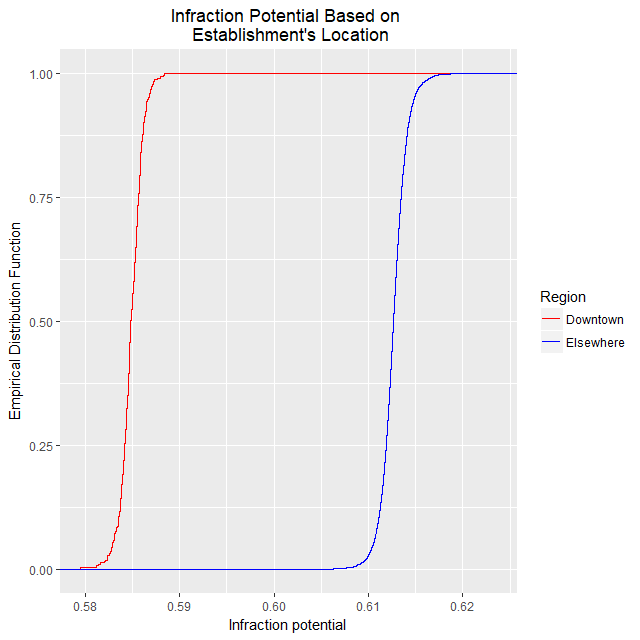
\includegraphics[height=8cm]{Infraction_Potential}
\caption{Infraction Potential Based on Establishment's Location}
\label{fig:Infraction_Potential_Based_on_Location}
\end{figure}

On the other hand, as shown in Table~\ref{table:delta_lambda_ci}, the central 95\% credible interval for the difference between two parameters, $\delta_i$ and $\lambda_i$, suggests that there is a statistically significant "Entertainment District effect" on the "rate" at which the infraction takes place for any of the establishments, given "potential." As shown in Figure~\ref{fig:ECDF of Expected Count of Infraction}, more than 90\% of the establishments outside the entertainment district will have less than 2 infractions found in the case of non-compliance. In other words, these establishments are most likely to have only one infraction, if any. On the other hand, only 10\% of those establishments in the entertainment district will be found with only one infraction and, in almost all cases, they will have two counts of non-compliance.

\begin{table}[ht]
\caption{Excerpt of the Credible Interval of the Difference, delta - lambda} % title of Table
\centering % used for centering table
\begin{tabular}{c c c} % centered columns (3 columns)
\hline\hline %inserts double horizontal lines
 & Lower C.I & Upper C.I. \\ [1ex] % inserts table
%heading
\hline % inserts single horizontal line
1 & -0.2240521 & -0.3216410 \\ % inserting body of the table
2 & -0.7112872 & -0.8171107 \\ 
3 & -1.4653769 & -1.5467638 \\
4 & -1.8081946 & -1.8972183 \\
5 & -0.6031131 & -0.7130676 \\ [1ex] % [1ex] adds vertical space
\hline %inserts single line
\end{tabular}
\label{table:delta_lambda_ci} % is used to refer this table in the text
\end{table}

\begin{figure}[H]
\centering
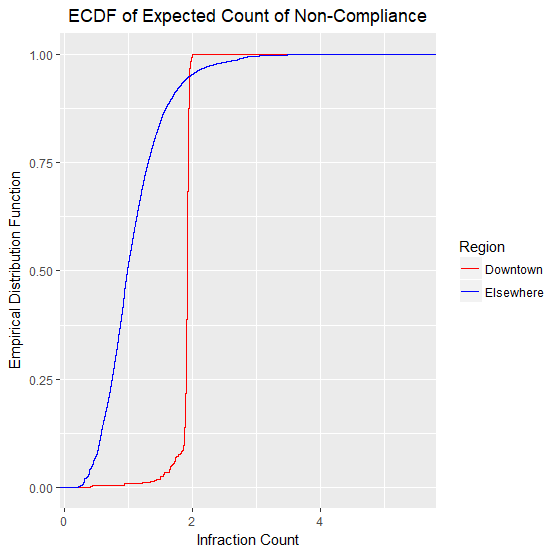
\includegraphics[height=8cm]{ECDF}
\caption{ECDF of Expected Count of Infraction given Potential}
\label{fig:ECDF of Expected Count of Infraction}
\end{figure}

This effect becomes more evident when we take the minimum required inspections into account. Each year every establishment has to be inspected a certain number of times, depending on their location, type of service provided, previous compliance history and other criteria. Hence, it makes sense to determine the "potential" and "count" of infractions for each establishment during those minimum required inspections. 

The binomial distribution is used to determine the "potential" for the establishment i to observe an "infraction" during "N" number of minimum required inspections, in which each inspection independently have the potential, "$\theta_i$", to observe an infraction. For the "count", the sum of independent and identically distributed Poisson random variables is used. Each inspection ij, if observed with any infraction, has an average of "$\psi_ij$" number of infractions observed. The sum of "N" iid Poisson random variable is simply the Poisson random variable with the rate parameter $N*\psi_{i}$. 

\begin{figure}[H]
\centering
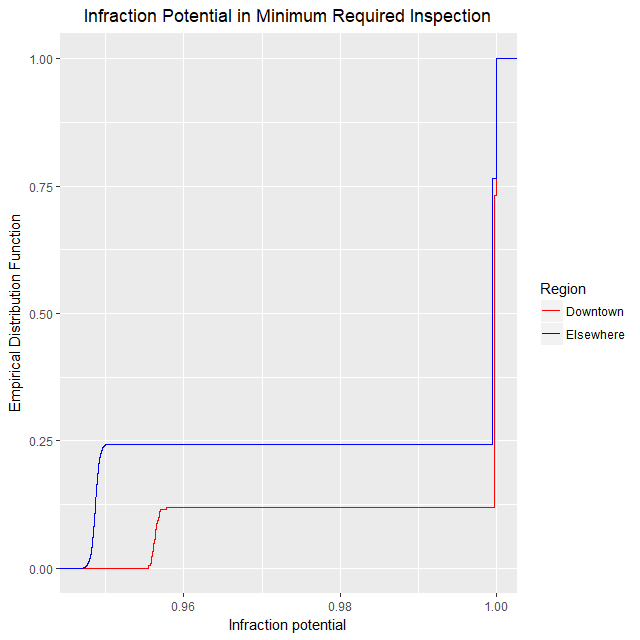
\includegraphics[height=8cm]{ECDF_min_potential}
\caption{ECDF of Infraction Potential during Minimum Required Inspections}
\label{fig:ECDF_min_potential}
\end{figure}

\begin{figure}[H]
\centering
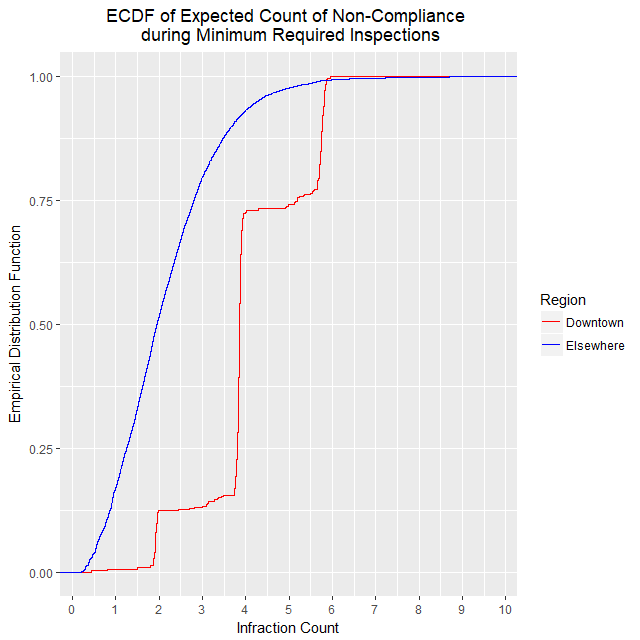
\includegraphics[height=8cm]{ecdf_min_count}
\caption{ECDF of Expected Count of Non-Compliance during Minimum Required Inspections}
\label{fig:ECDF_min_count}
\end{figure}

As shown in Figure~\ref{fig:ECDF_min_potential}, the potential to observe any infraction during minimum required inspections is negligible between two groups of establishments. That is, about 25\% of establishments outside the entertainment district have 95\% or less chance of being observed with an infraction during the minimum required inspections and the rest have close to 100\% probability of being observed so, whereas only about 10\% of establishments in the said district have 95.5\% or less change of being observed with an infraction during the minimum required inspections and the rest have close to 100\% probability of being observed so. 

Similar to a single inspection case, the establishments in the entertainment district are likely to have more counts of the food safety regulations violated, if any, than those outside the district. As shown in  Figure~\ref{fig:ECDF_min_count}, approximately 10\% of establishments in the entertainment district have 2 or less counts of infractions during the minimum required inspections and approximately 65\% of establishments in the district have between 2 and 4 counts of infractions. On the other hand, about 50\% of establishments outside the region have 2 or less counts of infractions and about 30\% have between 2 and 4 counts of infractions. This clearly shows that even though the infraction potential is consistent across all regions of Toronto, the entertainment district tends to be less compliant to the food safety regulations in the case of non-compliance.

In short, the "Entertainment District effect" can be described as an aggravating factor. Even though the establishments in the entertainment district are, negligibly, less likely to infringe the food safety regulations than those outside the district, in the case of non-compliance, it is likely to have higher counts of infractions at these establishments.

%------------------------------------------------


%------------------------------------------------

\section{Conclusion}
We have described a Bayesian approach for fitting zero-inflated count data. The advantage of utilizing the Bayesian approach is in the interpretation of both the approach itself and the outcome it produces.  The zero-inflated Poisson model for the regulatory compliance at the inspection level allows for the inference related to the geographical significance on the "severity", in terms of counts of infractions, establishment's non-compliance. 

%----------------------------------------------------------------------------------------
%	REFERENCE LIST
%----------------------------------------------------------------------------------------

\begin{thebibliography}{99} % Bibliography - this is intentionally simple in this template
\bibitem[1]{Toronto}
The City of Toronto (2017).
\newblock Toronto Open Data Catalogue - Dinesafe
\newblock Retrieved May 4, 2017, from \url{https://www1.toronto.ca/wps/portal/contentonly?vgnextoid=b54a5f9cd70bb210VgnVCM1000003dd60f89RCRD&vgnextchannel=09c6e03bb8d1e310VgnVCM10000071d60f89RCRD}

\bibitem[2]{Gelman2007}
Gelman, A \& Hill, J. (2007).
\newblock Data Analysis Using Regression and Multilevel/Hierarchical Models, 158

\bibitem[3]{Lambert}
Lambert, D (1992).
\newblock Zero-inflated Poisson regression, with an application to
random defects in manufacturing. 
\newblock {\em Technometrics}, 34:1-14

\bibitem[4]{Mullahy}
Mullahy, J (1986).
\newblock Specification and testing of some modified count data models. 
\newblock {\em Journal of Econometrics}, 3:341-65.
 
\end{thebibliography}

%----------------------------------------------------------------------------------------
\newpage
\section*{Appendix}
\begin{figure}[H]
\centering
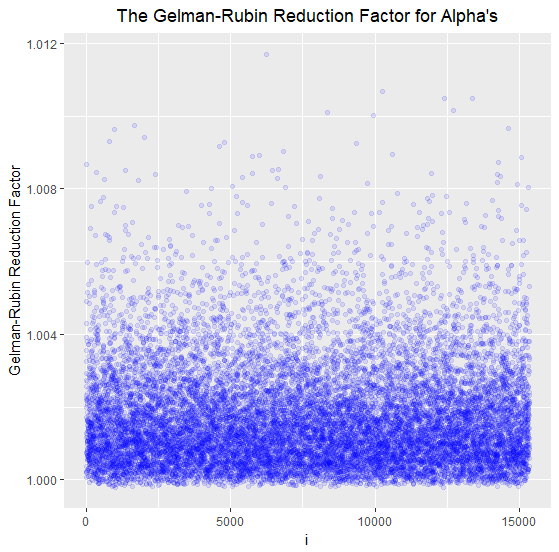
\includegraphics[height=8cm]{gelman_alpha_summary}
\caption{The Gelman-Rubin Reduction Factor for Alpha's}
\label{fig:gelman_alpha_summary}
\end{figure}

\begin{figure}[H]
\centering
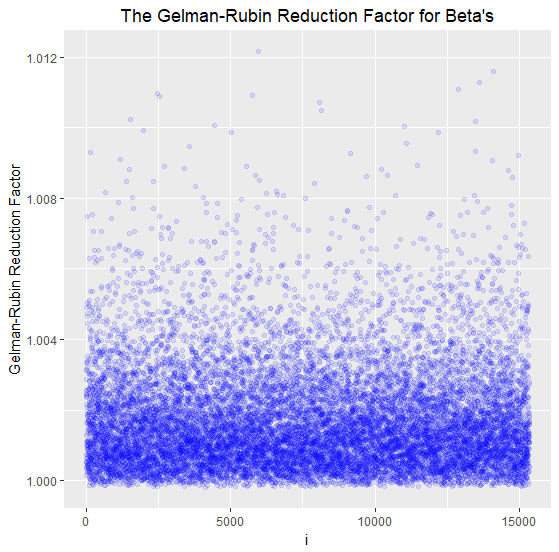
\includegraphics[height=8cm]{gelman_beta_summary}
\caption{The Gelman-Rubin Reduction Factor for Beta's}
\label{fig:gelman_beta_summary}
\end{figure}

\begin{figure}[H]
\centering
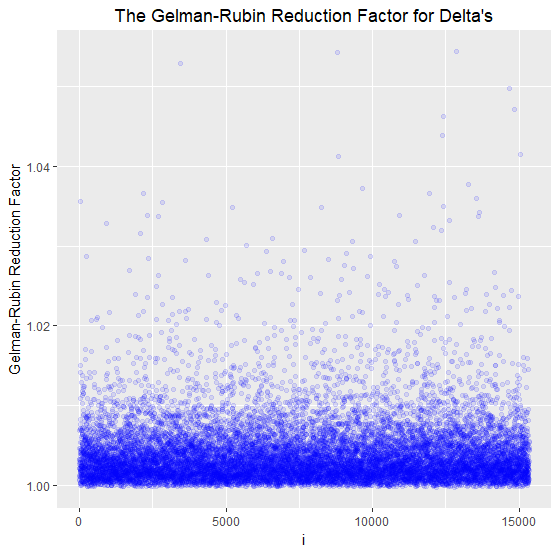
\includegraphics[height=8cm]{gelman_delta_summary}
\caption{The Gelman-Rubin Reduction Factor for Delta's}
\label{fig:gelman_delta_summary}
\end{figure}

\begin{figure}[H]
\centering
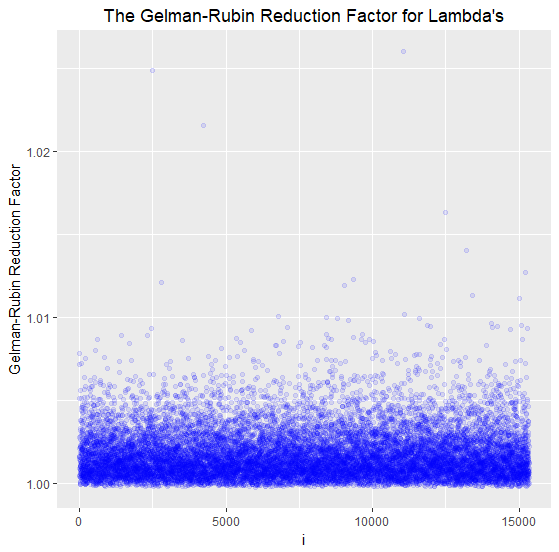
\includegraphics[height=8cm]{gelman_lambda_summary}
\caption{The Gelman-Rubin Reduction Factor for Lambda's}
\label{fig:gelman_lambda_summary}
\end{figure}


\end{document}
